%\pdfpageattr {/Group << /S /Transparency /I true /CS /DeviceRGB>>}
\documentclass[10pt, xcolor={usenames, dvipsnames}]{beamer}

\usepackage[french, english]{babel}
\usepackage[utf8]{inputenc}
\usepackage[T1]{fontenc}
\usepackage{upgreek,textgreek}
\usepackage{animate}

\usepackage{fontawesome}

\usepackage{fnpct}

\usepackage{pifont}
\newcommand{\cmark}{\ding{51}}
\newcommand{\xmark}{\ding{55}}

\usepackage{amsmath}
\usepackage{amssymb}

\usepackage{graphicx}
\usepackage{hyperref}
\usepackage[style=alphabetic, autocite=inline, firstinits=true, maxnames=2]{biblatex}
\bibliography{bibliographie}
%\renewcommand*{\bibfont}{\small}

\usepackage{makecell}
\usepackage{tabularx, booktabs}
\usepackage{tikz}
\definecolor{light-gray}{gray}{0.65}
\tikzset{fade on/.code={\only<#1>{\color{light-gray}}}}
\tikzset{hide on/.code={\only<#1>{\color{white}}}}
\tikzset{bold on/.code={\only<#1>{\bfseries}}}
\tikzset{
  opinvisible/.style={opacity=0.2},
  visible on/.style={alt={#1{}{opinvisible}}},
  alt/.code args={<#1>#2#3}{%
    \alt<#1>{\pgfkeysalso{#2}}{\pgfkeysalso{#3}} % \pgfkeysalso doesn't change the path
  },
}

\usetikzlibrary{plotmarks,shapes}
\usepackage{colortbl}
\usepackage{ulem}
\usepackage{multicol}
\usepackage[overlay]{textpos}
\usepackage{multirow}
\usepackage{ragged2e}
\usepackage{rotating}
\usepackage{fancybox}
\usepackage{ulem}
\usepackage{overpic}
\usepackage{enumerate}
\usepackage{xfrac}
\usepackage{pgfplots}

\usepackage{transparent}

\usepackage{epstopdf}
\usepackage{epsfig}


\newcommand{\REF}{\textcolor{purple}{REF}}
\newcommand{\GO}[1]{\textcolor{blue}{#1}}
\newcommand{\YES}[1]{\textcolor{green}{#1}}
\newcommand{\NO}[1]{\textcolor{red}{#1}}

\usetheme{metropolis}

\title{Breaking the Scalability Barrier of Causal Broadcast for Large and Dynamic Systems}
\author{\textbf{Brice N{\'e}delec}, Pascal Molli, and Achour Most{\'e}faoui}
\date{SRDS'18, October 02--05}
\institute{
  \vspace{4em}
  \begin{center}
    \begin{minipage}{0.48\textwidth}
      \centering
      
\includegraphics[width=0.5\textwidth]{logos/nantes.png}
    \end{minipage}
    \begin{minipage}{0.48\textwidth}
      \centering
      
\includegraphics[width=0.3\textwidth]{logos/ls2n.jpg}
    \end{minipage}
  \end{center}
}



\begin{document}

\maketitle

\begin{frame}{Introduction}

  Causal broadcast is the core of many distributed applications such as
  distributed social networks, distributed collaborative software, or
  distributed data stores.

  \vspace{3em}
  
    \begin{minipage}{0.19\textwidth}
      \centering
      
\includegraphics[width=0.7\textwidth]{logos/facebook.png}
    \end{minipage}
    \begin{minipage}{0.19\textwidth}
      \centering
      
\includegraphics[width=0.7\textwidth]{logos/mastodon.png}
    \end{minipage}
    \begin{minipage}{0.19\textwidth}
      \centering
      
\includegraphics[width=0.7\textwidth]{logos/telegram.png}
    \end{minipage}    
    \begin{minipage}{0.19\textwidth}
      \centering
      
\includegraphics[width=0.7\textwidth]{logos/google.png}
    \end{minipage}
    \begin{minipage}{0.19\textwidth}
      \centering
      
\includegraphics[width=0.8\textwidth]{logos/riak.png}
    \end{minipage}

\end{frame}


\begin{frame}{Causal broadcast}

  Causal broadcast is a reliable broadcast that ensures a specific ordering
  among message deliveries. 
  
  \begin{definition}[Lamport's Happen before]
    Happen before is a transitive, irreflexive, and antisymmetric relation
    $\rightarrow$ that defines a strict partial orders of events.  The sending
    of a message always precedes its receipt.
  \end{definition}

  \vspace{2em}

  \begin{definition}[Causal order]
    The delivery order of messages follows the happen before relationships of the
    corresponding broadcasts. $\forall A,\,B,\,C,\,
    b_A(m) \rightarrow b_B(m') \implies d_C(m) \rightarrow d_C(m')$
  \end{definition}

  \textit{When Alice comments on Bob's picture, everyone sees Alice's comment
    after Bob's picture.}

\end{frame}


\begin{frame}{A. Large scale systems: \NO{\xmark}}

  Piggybacking a vector of Lamport's clocks allows processes to order message
  deliveries.

  \begin{minipage}{0.32\textwidth}
    \begin{center}
      
\begin{tikzpicture}[scale=1]
  
  \small
  
  \newcommand\X{210/5pt};
  \newcommand\Y{30pt};
  
  % \draw[->] ( -0.5*\X, 0.5*\Y) -- ( -5+0*\X, 0*\Y);
  % \draw[->] ( -0.5*\X, 0*\Y) -- ( -5+0*\X, 0*\Y);
  % \draw[->] ( -0.5*\X, -0.5*\Y) -- ( -5+0*\X, 0*\Y);  

  \draw[fill=white] (0*\X, 0*\Y) node{\GO{\textbf{A}}} +(-5pt, -5pt) rectangle +(5pt, 5pt);
  \draw (0*\X, 5+0*\Y) node[above]{\GO{$[1]$}};

  \draw[fill=white] (1*\X, -1*\Y) node{\textbf{B}} +(-5pt, -5pt) rectangle +(5pt, 5pt);
  \draw[fill=white] (2*\X,  0*\Y) node{\textbf{C}} +(-5pt, -5pt) rectangle +(5pt, 5pt);

  \draw[->](5+0*\X, 0*\Y) -- node[sloped, above]{\GO{$[1]a$}} (-5+1*\X, -1*\Y); %% A->B
  \draw[<-](5+0*\X, -5+0*\Y) -- (-5+1*\X, -5-1*\Y); %% A<-B

  \draw[->](5+0*\X, 5+0*\Y) node[above right]{~ ~ ~ ~\GO{$[1]a$}} --  (-5+2*\X, 5+0*\Y); % A->C
  \draw[<-](5+0*\X,  1.25+ 0*\Y) -- (-5+2*\X,  1.25+ 0*\Y); % A<-C
 
  \draw[<-](5+1*\X, -1*\Y) -- (-5+2*\X, 0*\Y); %% B<-C
  \draw[->](5+1*\X, -5-1*\Y) -- (-5+2*\X, -5+0*\Y); %% B->C

  % \draw[->](5+2*\X, 0*\Y) -- ( 2.5*\X, 0*\Y);
\end{tikzpicture}
    \end{center}
  \end{minipage}
  \begin{minipage}{0.32\textwidth}
    \vspace{1.35em}
    \begin{center}
      
\begin{tikzpicture}[scale=1]
  
  \small
  
  \newcommand\X{210/5pt};
  \newcommand\Y{30pt};
  
  % \draw[->] ( -0.5*\X, 0.5*\Y) -- ( -5+0*\X, 0*\Y);
  % \draw[->] ( -0.5*\X, 0*\Y) -- ( -5+0*\X, 0*\Y);
  % \draw[->] ( -0.5*\X, -0.5*\Y) -- ( -5+0*\X, 0*\Y);  

  \draw[fill=white] (0*\X, 0*\Y) node{\textbf{A}} +(-5pt, -5pt) rectangle +(5pt, 5pt);
  \draw (0*\X, 5+0*\Y) node[above]{$[1]$};
  \draw[fill=white] (1*\X, -1*\Y) node{\GO{\textbf{B}}} +(-5pt, -5pt) rectangle +(5pt, 5pt);
  \draw (1*\X, 5-1*\Y) node[above]{$a$};
  \draw (1*\X, -5-1*\Y) node[below]{\GO{$[1]$}};


  \draw[fill=white] (2*\X,  0*\Y) node{\textbf{C}} +(-5pt, -5pt) rectangle +(5pt, 5pt);


  \draw[->](5+0*\X, 0*\Y) -- (-5+1*\X, -1*\Y); %% A->B
  \draw[<-](5+0*\X, -5+0*\Y) -- (-5+1*\X, -5-1*\Y); %% A<-B

  \draw[->](5+0*\X, 5+0*\Y) node[above right]{~ ~ ~ ~$[1]a$} --  (-5+2*\X, 5+0*\Y); % A->C
  \draw[<-](5+0*\X,  1.25+ 0*\Y) -- (-5+2*\X,  1.25+ 0*\Y); % A<-C
 
  \draw[<-](5+1*\X, -1*\Y) -- (-5+2*\X, 0*\Y); %% B<-C
  \draw[->](5+1*\X, -5-1*\Y) -- (-5+2*\X, -5+0*\Y); %% B->C

  % \draw[->](5+2*\X, 0*\Y) -- ( 2.5*\X, 0*\Y);
\end{tikzpicture}
    \end{center}
  \end{minipage}
  \begin{minipage}{0.32\textwidth}
    \vspace{1.35em}
    \begin{center}
      
\begin{tikzpicture}[scale=1]
  
  \small
  
  \newcommand\X{210/5pt};
  \newcommand\Y{30pt};
  
  % \draw[->] ( -0.5*\X, 0.5*\Y) -- ( -5+0*\X, 0*\Y);
  % \draw[->] ( -0.5*\X, 0*\Y) -- ( -5+0*\X, 0*\Y);
  % \draw[->] ( -0.5*\X, -0.5*\Y) -- ( -5+0*\X, 0*\Y);  

  \draw[fill=white] (0*\X, 0*\Y) node{\textbf{A}} +(-5pt, -5pt) rectangle +(5pt, 5pt);
  \draw (0*\X, 5+0*\Y) node[above]{$[1]$};
  \draw[fill=white] (1*\X, -1*\Y) node{\GO{\textbf{B}}} +(-5pt, -5pt) rectangle +(5pt, 5pt);
  \draw (1*\X, -5-1*\Y) node[below]{\GO{$[1,\,1]$}};
  \draw[fill=white] (2*\X,  0*\Y) node{\textbf{C}} +(-5pt, -5pt) rectangle +(5pt, 5pt);
%  \draw (1*\X, 5-1*\Y) node[above]{$a$};

  \draw[->](5+0*\X, 0*\Y) -- (-5+1*\X, -1*\Y); %% A->B
  \draw[<-](5+0*\X, -5+0*\Y) -- node[sloped, below]{\GO{$[1,\,1]b$}}
  (-5+1*\X, -5-1*\Y); %% A<-B

  \draw[->](5+0*\X, 5+0*\Y) -- node[above right]{~ ~$\pmb{[1]}a$} (-5+2*\X, 5+0*\Y); % A->C
  \draw[<-](5+0*\X,  1.25+ 0*\Y) -- (-5+2*\X,  1.25+ 0*\Y); % A<-C
 
  \draw[<-](5+1*\X, -1*\Y) -- (-5+2*\X, 0*\Y); %% B<-C
  \draw[->](5+1*\X, -5-1*\Y) --  node[sloped, below]{$\GO{\pmb{[1,\,1]}b}$} (-5+2*\X, -5+0*\Y); %% B->C

  % \draw[->](5+2*\X, 0*\Y) -- ( 2.5*\X, 0*\Y);
\end{tikzpicture}
    \end{center}
  \end{minipage}

  
  \vspace{1em}

  However, the size of vectors increases linearly and monotonically with the
  number of processes that ever broadcast a message. It does not scale in large
  systems.

\end{frame}


\begin{frame}{B. Static systems: \YES{\cmark}}
  
  \vspace{2em}
  
  Simply broadcast and forward each message exactly once using all outgoing FIFO
  links and you have causal broadcast\footnote{Friedman et al. Causal ordering
    in deterministic overlay networks.}.

  \begin{minipage}{0.32\textwidth}
    \begin{center}
      % \subfloat[Part A][\label{fig:generalsolveA}Process~A broadcasts $a$.]
      
\begin{tikzpicture}[scale=1]
  
  \small
  
  \newcommand\X{210/5pt};
  \newcommand\Y{30pt};
  
  % \draw[->] ( -0.5*\X, 0.5*\Y) -- ( -5+0*\X, 0*\Y);
  % \draw[->] ( -0.5*\X, 0*\Y) -- ( -5+0*\X, 0*\Y);
  % \draw[->] ( -0.5*\X, -0.5*\Y) -- ( -5+0*\X, 0*\Y);  

  \draw[fill=white] (0*\X, 0*\Y) node{\GO{\textbf{A}}} +(-5pt, -5pt) rectangle +(5pt, 5pt);
  \draw[fill=white] (1*\X, -1*\Y) node{\textbf{B}} +(-5pt, -5pt) rectangle +(5pt, 5pt);
  \draw[fill=white] (2*\X,  0*\Y) node{\textbf{C}} +(-5pt, -5pt) rectangle +(5pt, 5pt);

  \draw[->](5+0*\X, 0*\Y) -- node[sloped, above]{\GO{$a$}} (-5+1*\X, -1*\Y); %% A->B
  \draw[<-](5+0*\X, -5+0*\Y) -- (-5+1*\X, -5-1*\Y); %% A<-B

  \draw[->](5+0*\X, 5+0*\Y) node[above right]{\GO{$\,\,a$}} --  (-5+2*\X, 5+0*\Y); % A->C
  \draw[<-](5+0*\X,  1.25+ 0*\Y) -- (-5+2*\X,  1.25+ 0*\Y); % A<-C
 
  \draw[<-](5+1*\X, -1*\Y) -- (-5+2*\X, 0*\Y); %% B<-C
  \draw[->](5+1*\X, -5-1*\Y) -- (-5+2*\X, -5+0*\Y); %% B->C

  % \draw[->](5+2*\X, 0*\Y) -- ( 2.5*\X, 0*\Y);
\end{tikzpicture}
    \end{center}
  \end{minipage}
  \begin{minipage}{0.32\textwidth}
    \begin{center}
      % \subfloat[Part B][\label{fig:generalsolveB}Process~B receives and 
      % delivers $a$. Process~B forwards $a$ using its FIFO links.]
      
\begin{tikzpicture}[scale=1]
  
  \small
  
  \newcommand\X{210/5pt};
  \newcommand\Y{30pt};
  
  % \draw[->] ( -0.5*\X, 0.5*\Y) -- ( -5+0*\X, 0*\Y);
  % \draw[->] ( -0.5*\X, 0*\Y) -- ( -5+0*\X, 0*\Y);
  % \draw[->] ( -0.5*\X, -0.5*\Y) -- ( -5+0*\X, 0*\Y);  

  \draw[fill=white] (0*\X, 0*\Y) node{\textbf{A}} +(-5pt, -5pt) rectangle +(5pt, 5pt);
  \draw[fill=white] (1*\X, -1*\Y) node{\GO{\textbf{B}}} +(-5pt, -5pt) rectangle +(5pt, 5pt);
  \draw[fill=white] (2*\X,  0*\Y) node{\textbf{C}} +(-5pt, -5pt) rectangle +(5pt, 5pt);
  \draw (1*\X, 5-1*\Y) node[above]{$a$};

  \draw[->](5+0*\X, 0*\Y) -- (-5+1*\X, -1*\Y); %% A->B
  \draw[<-](5+0*\X, -5+0*\Y) -- node[sloped, below right]{\GO{$\,\,a$}} (-5+1*\X, -5-1*\Y); %% A<-B

  \draw[->](5+0*\X, 5+0*\Y) -- node[above left]{$a$} (-5+2*\X, 5+0*\Y); % A->C
  \draw[<-](5+0*\X,  1.25+ 0*\Y) -- (-5+2*\X,  1.25+ 0*\Y); % A<-C
 
  \draw[<-](5+1*\X, -1*\Y) -- (-5+2*\X, 0*\Y); %% B<-C
  \draw[->](5+1*\X, -5-1*\Y) --  node[sloped, below left]{\GO{$a\,\,$}} (-5+2*\X, -5+0*\Y); %% B->C

  % \draw[->](5+2*\X, 0*\Y) -- ( 2.5*\X, 0*\Y);
\end{tikzpicture}
    \end{center}
  \end{minipage}
  \begin{minipage}{0.32\textwidth}
    \begin{center}
      % \subfloat[Part C][\label{fig:generalsolveC}Process~B broadcasts $b$.]
      
\begin{tikzpicture}[scale=1]
  
  \small
  
  \newcommand\X{210/5pt};
  \newcommand\Y{30pt};
  
  % \draw[->] ( -0.5*\X, 0.5*\Y) -- ( -5+0*\X, 0*\Y);
  % \draw[->] ( -0.5*\X, 0*\Y) -- ( -5+0*\X, 0*\Y);
  % \draw[->] ( -0.5*\X, -0.5*\Y) -- ( -5+0*\X, 0*\Y);  

  \draw[fill=white] (0*\X, 0*\Y) node{\textbf{A}} +(-5pt, -5pt) rectangle +(5pt, 5pt);
  \draw[fill=white] (1*\X, -1*\Y) node{\GO{\textbf{B}}} +(-5pt, -5pt) rectangle +(5pt, 5pt);
  \draw[fill=white] (2*\X,  0*\Y) node{\textbf{C}} +(-5pt, -5pt) rectangle +(5pt, 5pt);
%  \draw (1*\X, 5-1*\Y) node[above]{$a$};

  \draw[->](5+0*\X, 0*\Y) -- (-5+1*\X, -1*\Y); %% A->B
  \draw[<-](5+0*\X, -5+0*\Y) -- node[sloped, below]{$a\,\,\,\,\,\,$ \GO{$b$}}
  (-5+1*\X, -5-1*\Y); %% A<-B

  \draw[->](5+0*\X, 5+0*\Y) -- node[above]{$a$} (-5+2*\X, 5+0*\Y); % A->C
  \draw[<-](5+0*\X,  1.25+ 0*\Y) -- (-5+2*\X,  1.25+ 0*\Y); % A<-C
 
  \draw[<-](5+1*\X, -1*\Y) -- (-5+2*\X, 0*\Y); %% B<-C
  \draw[->](5+1*\X, -5-1*\Y) --  node[sloped, below]{$\GO{b}$$\,\,\,\,\,\,a$} (-5+2*\X, -5+0*\Y); %% B->C

  % \draw[->](5+2*\X, 0*\Y) -- ( 2.5*\X, 0*\Y);
\end{tikzpicture}
    \end{center}
  \end{minipage}
  
  \begin{center}
  \begin{minipage}{0.35\textwidth}
    \begin{center}
    % \subfloat[Part D][\label{fig:generalsolveD}Process~A receives and 
    % delivers $b$. Process~A forwards $b$ using its FIFO links.]
      
\begin{tikzpicture}[scale=1]
  
  \small
  
  \newcommand\X{210/5pt};
  \newcommand\Y{30pt};
  
  % \draw[->] ( -0.5*\X, 0.5*\Y) -- ( -5+0*\X, 0*\Y);
  % \draw[->] ( -0.5*\X, 0*\Y) -- ( -5+0*\X, 0*\Y);
  % \draw[->] ( -0.5*\X, -0.5*\Y) -- ( -5+0*\X, 0*\Y);  

  \draw[fill=white] (0*\X, 0*\Y) node{\GO{\textbf{A}}} +(-5pt, -5pt) rectangle +(5pt, 5pt);
  \draw (-5 + 0*\X, 0*\Y) node[left]{$b$};
  \draw[fill=white] (1*\X, -1*\Y) node{\textbf{B}} +(-5pt, -5pt) rectangle +(5pt, 5pt);
  \draw[fill=white] (2*\X,  0*\Y) node{\textbf{C}} +(-5pt, -5pt) rectangle +(5pt, 5pt);
%  \draw (1*\X, 5-1*\Y) node[above]{$a$};

  \draw[->](5+0*\X, 0*\Y) --
  node[sloped, above left]{$\GO{b}\,\,\,$}
  (-5+1*\X, -1*\Y); %% A->B
  \draw[<-](5+0*\X, -5+0*\Y) -- (-5+1*\X, -5-1*\Y); %% A<-B

  \draw[->](5+0*\X, 5+0*\Y) node[above right]{$\GO{b}$}-- node[above right]{$a$} (-5+2*\X, 5+0*\Y); % A->C
  \draw[<-](5+0*\X,  1.25+ 0*\Y) -- (-5+2*\X,  1.25+ 0*\Y); % A<-C
 
  \draw[<-](5+1*\X, -1*\Y) -- (-5+2*\X, 0*\Y); %% B<-C
  \draw[->](5+1*\X, -5-1*\Y) --  node[sloped, below]{$b\,\,\,\,\,\,a$} (-5+2*\X, -5+0*\Y); %% B->C

  % \draw[->](5+2*\X, 0*\Y) -- ( 2.5*\X, 0*\Y);
\end{tikzpicture}
    \end{center}
  \end{minipage}
  \begin{minipage}{0.35\textwidth}
    \begin{center}
    % \hspace{40pt}
    % \subfloat[Part E][\label{fig:generalsolveE}Process~C cannot receive $b$
    % without having received $a$ beforehand.]
      
\begin{tikzpicture}[scale=1]
  
  \small
  
  \newcommand\X{210/5pt};
  \newcommand\Y{30pt};
  
  % \draw[->] ( -0.5*\X, 0.5*\Y) -- ( -5+0*\X, 0*\Y);
  % \draw[->] ( -0.5*\X, 0*\Y) -- ( -5+0*\X, 0*\Y);
  % \draw[->] ( -0.5*\X, -0.5*\Y) -- ( -5+0*\X, 0*\Y);  

  \draw[fill=white] (0*\X, 0*\Y) node{\textbf{A}} +(-5pt, -5pt) rectangle +(5pt, 5pt);
  \draw[fill=white] (1*\X, -1*\Y) node{\textbf{B}} +(-5pt, -5pt) rectangle +(5pt, 5pt);
  \draw[fill=white] (2*\X,  0*\Y) node{\textbf{C}} +(-5pt, -5pt) rectangle +(5pt, 5pt);

  \draw[->](5+0*\X, 0*\Y) -- (-5+1*\X, -1*\Y); %% A->B
  \draw[<-](5+0*\X, -5+0*\Y) -- (-5+1*\X, -5-1*\Y); %% A<-B

  \draw[->](5+0*\X, 5+0*\Y) -- (-5+2*\X, 5+0*\Y) node[above left]{$\GO{\pmb{b\,a}}\,\,$}; % A->C
  \draw[<-](5+0*\X,  1.25+ 0*\Y) -- (-5+2*\X,  1.25+ 0*\Y); % A<-C
 
  \draw[<-](5+1*\X, -1*\Y) -- (-5+2*\X, 0*\Y); %% B<-C
  \draw[->](5+1*\X, -5-1*\Y) -- node[sloped, below right]{$\,\,\,\,\,\GO{\pmb{b\,a}}$} (-5+2*\X, -5+0*\Y); %% B->C

  % \draw[->](5+2*\X, 0*\Y) -- ( 2.5*\X, 0*\Y);
\end{tikzpicture}
    % \caption{\label{fig:generalsolve}Causal broadcast~\cite{friedman2004causal}
    %   ensures causal order.}
    \end{center}
  \end{minipage}
  \end{center}

  Propagation ensures causal order by design. It is very efficient, for message
  overhead remains constant $O(1)$.

  \vspace{2em}

\end{frame}

\begin{frame}{B. Large scale static systems: \YES{\cmark}}

  Each process has a partial view much smaller than the actual system size and
  efficiently propagates messages using gossiping.

  \begin{center}
    
\begin{tikzpicture}[scale=0.65]

  \small
  
  \newcommand\X{210/5pt};
  \newcommand\Y{30pt};
  
  \draw[->] ( -1*\X, 1*\Y) -- ( -5+0*\X, 0*\Y);
  \draw[->] ( -1*\X, 0*\Y) node[anchor=east, align=center]{Rest\\of the\\network} -- ( -5+0*\X, 0*\Y);
  \draw[->] ( -1*\X, -1*\Y) -- ( -5+0*\X, 0*\Y);

  \draw[<-] ( 5*\X, 1*\Y) -- ( 5+4*\X, 0*\Y);
  \draw[<-] ( 5*\X, 0*\Y) node[anchor=west, align=center]{Rest\\of the\\network}-- ( 5+4*\X, 0*\Y);
  \draw[<-] ( 5*\X, -1*\Y) -- ( 5+4*\X, 0*\Y);


  \draw[fill=white] (0*\X, 0*\Y) node{\textbf{A}} +(-5pt, -5pt) rectangle +(5pt, 5pt);

  \draw[fill=white] (1*\X, -1*\Y) node{\textbf{B}} +(-5pt, -5pt) rectangle +(5pt, 5pt);

  \draw[fill=white] (2*\X, -2*\Y) node{\textbf{E}} +(-5pt, -5pt) rectangle +(5pt, 5pt);
  \draw[fill=white] (2*\X,  0*\Y) node{\textbf{D}} +(-5pt, -5pt) rectangle +(5pt, 5pt);
  \draw[fill=white] (2*\X,  2*\Y) node{\textbf{C}} +(-5pt, -5pt) rectangle +(5pt, 5pt);

  \draw[fill=white] (4*\X, 0*\Y) node{\textbf{F}} +(-5pt, -5pt) rectangle +(5pt, 5pt);

  \draw[->](5+0*\X, 0*\Y) -- node[sloped, above]{\GO{\pmb{$a'\,a$}}} (-5+2*\X,  2*\Y); %% A->E
  \draw[->](5+0*\X, 0*\Y) -- node[sloped, above]{\GO{\pmb{$a'\,a$}}} (-5+1*\X, -1*\Y); %% A->B

  \draw[->](5+1*\X, -1*\Y) -- node[sloped, above]{$\pmb{a'}\,b\,\pmb{a}$} (-5+2*\X, 0*\Y); %% B->D
  \draw[->](5+1*\X, -1*\Y) -- node[sloped, above]{$\pmb{a'}\,b\,\pmb{a}$} (-5+2*\X, -2*\Y); %% B->C

  \draw[->](5+2*\X,  2*\Y) -- node[sloped, above]{$c\,\GO{\pmb{a'\,a}}$} (-5+4*\X, 0*\Y); %% E->F
  \draw[->](5+2*\X,  0*\Y) -- node[sloped, above]{$\GO{\pmb{a'}}\,b\,\GO{\pmb{a}}\,d$} (-5+4*\X, 0*\Y); %% D->F
  \draw[->](5+2*\X, -2*\Y) -- node[sloped, above]{$\GO{\pmb{a'}}\,b\,\,e'\,e\,\GO{\pmb{a}}$} (-5+4*\X, 0*\Y); %% C->F

  


\end{tikzpicture}
  \end{center}

  Gossiping is already mandatory for large scale systems. It is not an
  additional overhead of causal broadcast.

\end{frame}



\begin{frame}{B. But dynamic systems: \NO{\xmark}}

  New links may act as shortcut for new messages impairing causal order.

  \begin{minipage}{0.32\textwidth}
    \vspace{1pt}
    \begin{center}
      % \subfloat[Part A][\label{fig:generalsolveA}Process~A broadcasts $a$.]
      
\begin{tikzpicture}[scale=0.75]
  
  \small
  
  \newcommand\X{210/5pt};
  \newcommand\Y{30pt};
  
  \draw[->] ( -0.5*\X, 0.5*\Y) -- ( -5+0*\X, 0*\Y);
  \draw[->] ( -0.5*\X, 0*\Y) -- ( -5+0*\X, 0*\Y);
  \draw[->] ( -0.5*\X, -0.5*\Y) -- ( -5+0*\X, 0*\Y);  

  \draw[fill=white] (0*\X, 0*\Y) node{\GO{\textbf{A}}} +(-5pt, -5pt) rectangle +(5pt, 5pt);
  \draw[fill=white] (1*\X, -1*\Y) node{\textbf{B}} +(-5pt, -5pt) rectangle +(5pt, 5pt);
  \draw[fill=white] (2*\X,  0*\Y) node{\textbf{D}} +(-5pt, -5pt) rectangle +(5pt, 5pt);

  \draw[->](5+0*\X, 0*\Y) -- node[sloped, above left]{\GO{$a$}} (-5+1*\X, -1*\Y); %% A->B
  \draw[->](5+1*\X, -1*\Y) -- (-5+2*\X, 0*\Y); %% B->D

  \draw[->](5+2*\X, 0*\Y) -- ( 2.5*\X, 0*\Y);
\end{tikzpicture}
    \end{center}
  \end{minipage}
  \begin{minipage}{0.32\textwidth}
    \vspace{1pt}
    \begin{center}
      % \subfloat[Part B][\label{fig:generalsolveB}Process~B receives and 
      % delivers $a$. Process~B forwards $a$ using its FIFO links.]
      
\begin{tikzpicture}[scale=0.75]
  
  \small
  
  \newcommand\X{210/5pt};
  \newcommand\Y{30pt};
  
  \draw[->] ( -0.5*\X, 0.5*\Y) -- ( -5+0*\X, 0*\Y);
  \draw[->] ( -0.5*\X, 0*\Y) -- ( -5+0*\X, 0*\Y);
  \draw[->] ( -0.5*\X, -0.5*\Y) -- ( -5+0*\X, 0*\Y);  

  \draw[fill=white] (0*\X, 0*\Y) node{\textbf{A}} +(-5pt, -5pt) rectangle +(5pt, 5pt);
  \draw[fill=white] (1*\X, -1*\Y) node{\textbf{B}} +(-5pt, -5pt) rectangle +(5pt, 5pt);
  \draw[fill=white] (2*\X,  0*\Y) node{\textbf{D}} +(-5pt, -5pt) rectangle +(5pt, 5pt);

  \draw[->](5+0*\X, 0*\Y) -- node[sloped, above right]{$a$} (-5+1*\X, -1*\Y); %% A->B
  \draw[->](5+1*\X, -1*\Y) -- (-5+2*\X, 0*\Y); %% B->D

  \draw[->, color=blue] (5+0*\X, 0*\Y) -- (-5+2*\X, 0*\Y);

  \draw[->](5+2*\X, 0*\Y) -- ( 2.5*\X, 0*\Y);
\end{tikzpicture}
    \end{center}
  \end{minipage}
  \begin{minipage}{0.32\textwidth}
    \begin{center}
      % \subfloat[Part C][\label{fig:generalsolveC}Process~B broadcasts $b$.]
      
\begin{tikzpicture}[scale=0.75]
  
  \small
  
  \newcommand\X{210/5pt};
  \newcommand\Y{30pt};
  
  \draw[->] ( -0.5*\X, 0.5*\Y) -- ( -5+0*\X, 0*\Y);
  \draw[->] ( -0.5*\X, 0*\Y) -- ( -5+0*\X, 0*\Y);
  \draw[->] ( -0.5*\X, -0.5*\Y) -- ( -5+0*\X, 0*\Y);  

  \draw[fill=white] (0*\X, 0*\Y) node{\GO{\textbf{A}}} +(-5pt, -5pt) rectangle +(5pt, 5pt);
  \draw[fill=white] (1*\X, -1*\Y) node{\textbf{B}} +(-5pt, -5pt) rectangle +(5pt, 5pt);
  \draw (1*\X, 5-1*\Y) node[anchor=south]{$a$};
  \draw[fill=white] (2*\X,  0*\Y) node{\textbf{D}} +(-5pt, -5pt) rectangle +(5pt, 5pt);

  \draw[->](5+0*\X, 0*\Y) -- node[sloped, above]{\GO{$a'$}} (-5+1*\X, -1*\Y); %% A->B
  \draw[->](5+1*\X, -1*\Y) -- (-5+2*\X, 0*\Y); %% B->D
  
  \draw[->] (5+0*\X, 0*\Y) -- node[anchor=south]{\NO{$a'$}} (-5+2*\X, 0*\Y); %% A->B

  \draw[->](5+2*\X, 0*\Y) -- ( 2.5*\X, 0*\Y);
\end{tikzpicture}
    \end{center}
  \end{minipage}
  
  \begin{center}
  \begin{minipage}{0.35\textwidth}
    \begin{center}
    % \subfloat[Part D][\label{fig:generalsolveD}Process~A receives and 
    % delivers $b$. Process~A forwards $b$ using its FIFO links.]
      
\begin{tikzpicture}[scale=0.75]
  
  \small
  
  \newcommand\X{210/5pt};
  \newcommand\Y{30pt};
  
  \draw[->] ( -0.5*\X, 0.5*\Y) -- ( -5+0*\X, 0*\Y);
  \draw[->] ( -0.5*\X, 0*\Y) -- ( -5+0*\X, 0*\Y);
  \draw[->] ( -0.5*\X, -0.5*\Y) -- ( -5+0*\X, 0*\Y);  

  \draw[fill=white] (0*\X, 0*\Y) node{\textbf{A}} +(-5pt, -5pt) rectangle +(5pt, 5pt);
  \draw[fill=white] (1*\X, -1*\Y) node{\textbf{B}} +(-5pt, -5pt) rectangle +(5pt, 5pt);
  \draw (1*\X, 5-1*\Y) node[anchor=south]{$a'$};
  \draw[fill=white] (2*\X,  0*\Y) node{\NO{\textbf{D}}} +(-5pt, -5pt) rectangle +(5pt, 5pt);
  \draw (2*\X, 5-0*\Y) node[anchor=south]{$\NO{\pmb{a'}}$};

  \draw[->](5+0*\X, 0*\Y) --  (-5+1*\X, -1*\Y); %% A->B
  \draw[->](5+1*\X, -1*\Y) -- node[sloped, above]{$b\,\pmb{a}$} (-5+2*\X, 0*\Y); %% B->D
  
  \draw[->] (5+0*\X, 0*\Y) -- (-5+2*\X, 0*\Y); %% A->B

  \draw[->](5+2*\X, 0*\Y) -- ( 2.5*\X, 0*\Y);

\end{tikzpicture}
    \end{center}
  \end{minipage}
  \begin{minipage}{0.35\textwidth}
    \begin{center}
    % \hspace{40pt}
    % \subfloat[Part E][\label{fig:generalsolveE}Process~C cannot receive $b$
    % without having received $a$ beforehand.]
      
\begin{tikzpicture}[scale=0.75]
  
  \small
  
  \newcommand\X{210/5pt};
  \newcommand\Y{30pt};
  
  \draw[->] ( -0.5*\X, 0.5*\Y) -- ( -5+0*\X, 0*\Y);
  \draw[->] ( -0.5*\X, 0*\Y) -- ( -5+0*\X, 0*\Y);
  \draw[->] ( -0.5*\X, -0.5*\Y) -- ( -5+0*\X, 0*\Y);  

  \draw[fill=white] (0*\X, 0*\Y) node{\textbf{A}} +(-5pt, -5pt) rectangle +(5pt, 5pt);
  \draw[fill=white] (1*\X, -1*\Y) node{\textbf{B}} +(-5pt, -5pt) rectangle +(5pt, 5pt);
  \draw[fill=white] (2*\X,  0*\Y) node{\textbf{C}} +(-5pt, -5pt) rectangle +(5pt, 5pt);
  \draw (2*\X, 5-0*\Y) node[anchor=south]{$b$};

  \draw[->](5+0*\X, 0*\Y) --  (-5+1*\X, -1*\Y); %% A->B
  \draw[->](5+1*\X, -1*\Y) -- node[sloped, above]{$a'$} (-5+2*\X, 0*\Y); %% B->D
  
  \draw[->] (5+0*\X, 0*\Y) -- (-5+2*\X, 0*\Y); %% A->B

  \draw[->](5+2*\X, 0*\Y) -- node[above right]{\NO{$\pmb{a\,a'}$}} ( 2.5*\X, 0*\Y);

\end{tikzpicture}
    % \caption{\label{fig:generalsolve}Causal broadcast~\cite{friedman2004causal}
    %   ensures causal order.}
    \end{center}
  \end{minipage}
  \end{center}  

  Not only Process~D fails to deliver messages in causal order but propagates the
  mistake to the rest of processes.

\end{frame}


\begin{frame}{Positioning}
  
  \begin{center}
  \begin{table}
    \begin{center}
      \caption{\label{table:comparison} Complexity of causal
        broadcast protocols.
        $N$ is the number of processes that ever broadcast a message.
        $W$ is the number of received messages awaiting delivery.
        $P$ is the number of delivered messages that are temporarily kept before
        being safely purged to forbid double delivery.%
        % $B$ is the number of delivered messages that are temporarily kept to
        % check the safety of new communication means.
      }
      %\setlength{\tabcolsep}{3pt} % General space between cols (6pt standard)
\small
\begin{tabularx}{0.95\columnwidth}{@{}Xcccc@{}}
%  \toprule
  & \makecell{dynamic\\systems} & \makecell{message\\overhead} & \makecell{local space\\consumption} &  \makecell{delivery\\execution time} \\ \cmidrule{2-5}
  vector-based & \YES{\cmark} & $O(\NO{N})$ & $O(\NO{N}+W\cdot\NO{N})$ & $O(W\cdot\NO{N})$ \\
  FIFO+forward & \NO{\xmark} & $O(1)$ & $O(P)$ & $O(1)$ \\ \hline\hline
%  objective & \cmark & $?<O(N)$ & $O(N)\leq \, ?$ & $? \leq O(W.N)$ \\ \hline\hline
  \textbf{our approach} & \textbf{\YES{\cmark}} & $\mathbf{O(1)}$ & $\mathbf{O(\NO{N})}$ & $\mathbf{O(1)}$ \\ 
%  \bottomrule
\end{tabularx}

%%% Local Variables:
%%% mode: latex
%%% TeX-master: "../paper"
%%% End:

    \end{center}
  \end{table}
  \end{center}

\end{frame}


\begin{frame}[standout]
  How do we keep the complexity of causal broadcast for large scale static
  systems in dynamic settings where processes can join, leave, or
  self-reconfigure at any time?
\end{frame}

\begin{frame}{Proposal: PC-broadcast}  

  PC-broadcast stands for Preventive Causal broadcast. 

  \vspace{2em}

  PC-broadcast prevents causal order
  violations by forbidding the usage of new links until proven safe. Each
  process uses all and only safe links for causal broadcast.
  
\end{frame}

\begin{frame}{Safe links}

  \begin{definition}[\label{def:safe}Safe link]
    A link from Process~A to Process~B is safe if and only if Process~B received
    or will receive all messages delivered by Process~A before receiving any
    message that Process~A will deliver:
    $safe_{AB} \equiv \forall m,\, m',\, d_A(m) \rightarrow s_{AB}(m') \implies
    r_B(m) \rightarrow r_{BA}(m')$
  \end{definition}

  \vspace{2em}

  Links start unsafe. The challenge is to make links safe using local knowledge
  only. Sending all delivered messages since the beginning makes safe links but
  is over-expansive: \NO{\xmark}. We will use few lightweight control messages
  that follow causal order: \YES{\cmark}.

\end{frame}


\begin{frame}{Control messages and buffering make safe links}
  
  \begin{enumerate}
  \item Sending a control message using safe link to the other process
    $\rightarrow$ will acknowledge the delivery of most of past messages
  \item Buffer all delivered messages $\rightarrow$ saves concurrent messages to
    safe link establishment
  \item Upon acknowledgment of the control message, send the buffer of
    concurrent messages
  \end{enumerate}


  \begin{minipage}{0.32\textwidth}
    \vspace{4pt}
    \begin{center}
      % \subfloat[Part A][\label{fig:generalsolveA}Process~A broadcasts $a$.]
      
\begin{tikzpicture}[scale=0.75]
  
  \small
  
  \newcommand\X{210/5pt};
  \newcommand\Y{30pt};
  
  \draw[->] ( -0.5*\X, 0.5*\Y) -- ( -5+0*\X, 0*\Y);
  \draw[->] ( -0.5*\X, 0*\Y) -- ( -5+0*\X, 0*\Y);
  \draw[->] ( -0.5*\X, -0.5*\Y) -- ( -5+0*\X, 0*\Y);  

  \draw[fill=white] (0*\X, 0*\Y) node{\textbf{A}} +(-5pt, -5pt) rectangle +(5pt, 5pt);
  \draw[fill=white] (1*\X, -1*\Y) node{\textbf{B}} +(-5pt, -5pt) rectangle +(5pt, 5pt);
  \draw[fill=white] (2*\X,  0*\Y) node{\textbf{D}} +(-5pt, -5pt) rectangle +(5pt, 5pt);

  \draw[->](5+0*\X, 0*\Y) -- node[sloped, above]{$a$} (-5+1*\X, -1*\Y); %% A->B
  \draw[->](5+1*\X, -1*\Y) -- (-5+2*\X, 0*\Y); %% B->D

  \draw[->](5+2*\X, 0*\Y) -- ( 2.5*\X, 0*\Y);
\end{tikzpicture}
    \end{center}
  \end{minipage}
  \begin{minipage}{0.32\textwidth}
    \begin{center}
      % \subfloat[Part B][\label{fig:generalsolveB}Process~B receives and 
      % delivers $a$. Process~B forwards $a$ using its FIFO links.]
      
\begin{tikzpicture}[scale=0.75]
  
  \small
  
  \newcommand\X{210/5pt};
  \newcommand\Y{30pt};
  
  \draw[->] ( -0.5*\X, 0.5*\Y) -- ( -5+0*\X, 0*\Y);
  \draw[->] ( -0.5*\X, 0*\Y) -- ( -5+0*\X, 0*\Y);
  \draw[->] ( -0.5*\X, -0.5*\Y) -- ( -5+0*\X, 0*\Y);  

  \draw[fill=white] (0*\X, 0*\Y) node{\textbf{A}} +(-5pt, -5pt) rectangle +(5pt, 5pt);
  \draw[fill=white] (1*\X, -1*\Y) node{\textbf{B}} +(-5pt, -5pt) rectangle +(5pt, 5pt);
  \draw (1*\X, 5-1*\Y) node[anchor=south]{$a$};
  \draw[fill=white] (2*\X,  0*\Y) node{\textbf{C}} +(-5pt, -5pt) rectangle +(5pt, 5pt);

  \draw[->](5+0*\X, 0*\Y) -- node[sloped, above]{\GO{$\pi$}} (-5+1*\X, -1*\Y); %% A->B
  \draw[->](5+1*\X, -1*\Y) -- (-5+2*\X, 0*\Y); %% B->D
  
  \draw[->, dashed, color=blue] (5+0*\X, 0*\Y) node[anchor=south west]{\GO{$[\,]$}} -- (-5+2*\X, 0*\Y); %% A->B

  \draw[->](5+2*\X, 0*\Y) -- ( 2.5*\X, 0*\Y);
\end{tikzpicture}
    \end{center}
  \end{minipage}
  \begin{minipage}{0.32\textwidth}
    \begin{center}
      % \subfloat[Part C][\label{fig:generalsolveC}Process~B broadcasts $b$.]
      
\begin{tikzpicture}[scale=0.75]
  
  \small
  
  \newcommand\X{210/5pt};
  \newcommand\Y{30pt};
  
  \draw[->] ( -0.5*\X, 0.5*\Y) -- ( -5+0*\X, 0*\Y);
  \draw[->] ( -0.5*\X, 0*\Y) -- ( -5+0*\X, 0*\Y);
  \draw[->] ( -0.5*\X, -0.5*\Y) -- ( -5+0*\X, 0*\Y);  

  \draw[fill=white] (0*\X, 0*\Y) node{\textbf{A}} +(-5pt, -5pt) rectangle +(5pt, 5pt);
  \draw[fill=white] (1*\X, -1*\Y) node{\textbf{B}} +(-5pt, -5pt) rectangle +(5pt, 5pt);
%  \draw (1*\X, 5-1*\Y) node[anchor=south]{$a$};
  \draw[fill=white] (2*\X,  0*\Y) node{\textbf{D}} +(-5pt, -5pt) rectangle +(5pt, 5pt);

  \draw[->](5+0*\X, 0*\Y) -- node[sloped, above]{$a'$} (-5+1*\X, -1*\Y); %% A->B
  \draw[->](5+1*\X, -1*\Y) -- node[sloped, above]{$\GO{\pi}\,b\,a$} (-5+2*\X, 0*\Y); %% B->D
  
  \draw[->, dashed] (5+0*\X, 0*\Y) node[anchor=south west]{$[\GO{a'}]$} --  (-5+2*\X, 0*\Y); %% A->B

  \draw[->](5+2*\X, 0*\Y) -- ( 2.5*\X, 0*\Y);
\end{tikzpicture}
    \end{center}
  \end{minipage}
  
  \begin{center}
  \begin{minipage}{0.35\textwidth}
    \begin{center}
    % \subfloat[Part D][\label{fig:generalsolveD}Process~A receives and 
    % delivers $b$. Process~A forwards $b$ using its FIFO links.]
      
\begin{tikzpicture}[scale=0.75]
  
  \small
  
  \newcommand\X{210/5pt};
  \newcommand\Y{30pt};
  
  \draw[->] ( -0.5*\X, 0.5*\Y) -- ( -5+0*\X, 0*\Y);
  \draw[->] ( -0.5*\X, 0*\Y) -- ( -5+0*\X, 0*\Y);
  \draw[->] ( -0.5*\X, -0.5*\Y) -- ( -5+0*\X, 0*\Y);  

  \draw[fill=white] (0*\X, 0*\Y) node{\textbf{A}} +(-5pt, -5pt) rectangle +(5pt, 5pt);
  \draw[fill=white] (1*\X, -1*\Y) node{\textbf{B}} +(-5pt, -5pt) rectangle +(5pt, 5pt);
  \draw (1*\X, 5-1*\Y) node[anchor=south]{$a'$};
  \draw[fill=white] (2*\X,  0*\Y) node{\textbf{C}} +(-5pt, -5pt) rectangle +(5pt, 5pt);
  \draw (2*\X, 5-0*\Y) node[anchor=south]{$\pi$};

  \draw[->](5+0*\X, 0*\Y) -- (-5+1*\X, -1*\Y); %% A->B
  \draw[->](5+1*\X, -1*\Y) -- (-5+2*\X, 0*\Y); %% B->D
  
  \draw[->, dashed] (5+0*\X, 0*\Y) node[anchor=south west]{$[a']$} --  (-5+2*\X, 0*\Y); %% A->B

  \draw[->, decorate, decoration={snake, amplitude=0.3mm}, color=blue](-5+2*\X, 5+0*\Y)
  to[out=180-25, in=25] node[sloped, above left]{\GO{$\rho$}}(0.65*\X, 10+0*\Y); 

  \draw[->](5+2*\X, 0*\Y) -- node[anchor=south]{$b\,a$}( 2.5*\X, 0*\Y);
\end{tikzpicture}
    \end{center}
  \end{minipage}
  \begin{minipage}{0.35\textwidth}
    \begin{center}
    \vspace{9pt}
    % \hspace{40pt}
    % \subfloat[Part E][\label{fig:generalsolveE}Process~C cannot receive $b$
    % without having received $a$ beforehand.]
      
\begin{tikzpicture}[scale=0.75]
  
  \small
  
  \newcommand\X{210/5pt};
  \newcommand\Y{30pt};
  
  \draw[->] ( -0.5*\X, 0.5*\Y) -- ( -5+0*\X, 0*\Y);
  \draw[->] ( -0.5*\X, 0*\Y) -- ( -5+0*\X, 0*\Y);
  \draw[->] ( -0.5*\X, -0.5*\Y) -- ( -5+0*\X, 0*\Y);  

  \draw[fill=white] (0*\X, 0*\Y) node{\textbf{A}} +(-5pt, -5pt) rectangle +(5pt, 5pt);
  \draw (0*\X, 5-0*\Y) node[anchor=south]{$\rho$};
  \draw[fill=white] (1*\X, -1*\Y) node{\textbf{B}} +(-5pt, -5pt) rectangle +(5pt, 5pt);
  \draw[fill=white] (2*\X,  0*\Y) node{\textbf{D}} +(-5pt, -5pt) rectangle +(5pt, 5pt);

  \draw[->](5+0*\X, 0*\Y) -- (-5+1*\X, -1*\Y); %% A->B
  \draw[->](5+1*\X, -1*\Y) -- node[sloped, above]{$a'$} (-5+2*\X, 0*\Y); %% B->D
  
  \draw[->, color=blue] (5+0*\X, 0*\Y)  -- node[anchor=south]{\GO{$a'$}} (-5+2*\X, 0*\Y); %% A->B

  \draw[->](5+2*\X, 0*\Y) -- node[anchor=south west]{$b$}( 2.5*\X, 0*\Y);
\end{tikzpicture}
    % \caption{\label{fig:generalsolve}Causal broadcast~\cite{friedman2004causal}
    %   ensures causal order.}
    \end{center}
  \end{minipage}
  \end{center}    

\end{frame}


\begin{frame}{The size of buffers may increase without bound}

  System conditions such as high latency, crashes, or unreliable communications
  may lead to unbounded growth of buffers.

  \begin{minipage}{0.98\textwidth}
    \begin{center}
      % \subfloat[Part A][\label{fig:generalsolveA}Process~A broadcasts $a$.]
      
\begin{tikzpicture}[scale=1]
  
  \small
  
  \newcommand\X{210/5pt};
  \newcommand\Y{30pt};
  
  \draw[->] ( -0.5*\X, 0.5*\Y) -- ( -5+0*\X, 0*\Y);
  \draw[->] ( -0.5*\X, 0*\Y) -- ( -5+0*\X, 0*\Y);
  \draw[->] ( -0.5*\X, -0.5*\Y) -- ( -5+0*\X, 0*\Y);  

  \draw[fill=white] (0*\X, 0*\Y) node{\textbf{A}} +(-5pt, -5pt) rectangle +(5pt, 5pt);
  \draw[fill=white] (1*\X, -1*\Y) node{\textbf{B}} +(-5pt, -5pt) rectangle +(5pt, 5pt);
  \draw (1*\X, 5-1*\Y) node[anchor=south]{\NO{$a''$}};
  \draw[fill=white] (2*\X,  0*\Y) node{\textbf{D}} +(-5pt, -5pt) rectangle +(5pt, 5pt);

  \draw[->, dashed] (5+0*\X, 0*\Y) -- (-5+2*\X, 0*\Y);

  \draw[->](5+0*\X, 0*\Y) node[anchor=south west]{$[y\, \ldots \,a'',\,a']$} -- node[sloped, above]{\NO{$y\, \dots$}} (-5+1*\X, -1*\Y); %% A->B
  \draw[->](5+1*\X, -1*\Y) -- node[sloped, above]{\NO{$a'\,\pi\,b\,a$}} (-5+2*\X, 0*\Y); %% B->D

  \draw[->](5+2*\X, 0*\Y) -- ( 2.5*\X, 0*\Y);
\end{tikzpicture}
    \end{center}
  \end{minipage}
  \begin{minipage}{0.98\textwidth}
    \begin{center}
      % \subfloat[Part B][\label{fig:generalsolveB}Process~B receives and 
      % delivers $a$. Process~B forwards $a$ using its FIFO links.]
      
\begin{tikzpicture}[scale=1]
  
  \small
  
  \newcommand\X{210/5pt};
  \newcommand\Y{30pt};
  
  \draw[->] ( -0.5*\X, 0.5*\Y) -- ( -5+0*\X, 0*\Y);
  \draw[->] ( -0.5*\X, 0*\Y) -- ( -5+0*\X, 0*\Y);
  \draw[->] ( -0.5*\X, -0.5*\Y) -- ( -5+0*\X, 0*\Y);  

  \draw[fill=white] (0*\X, 0*\Y) node{\textbf{A}} +(-5pt, -5pt) rectangle +(5pt, 5pt);
  \draw[fill=white] (1*\X, -1*\Y) node{\textbf{B}} +(-5pt, -5pt) rectangle +(5pt, 5pt);
  \draw (1*\X, 5-1*\Y) node[anchor=south]{$a''$};
  \draw[fill=white] (2*\X,  0*\Y) node{\textbf{C}} +(-5pt, -5pt) rectangle +(5pt, 5pt);

  \draw[->, dashed] (5+0*\X, 0*\Y) -- (-5+2*\X, 0*\Y);

  \draw[->](5+0*\X, 0*\Y) node[anchor=south west]{$[y\, \ldots \,a'',\,a']$} -- node[sloped, above]{$y\,\ldots$} (-5+1*\X, -1*\Y); %% A->B
  \draw[->](5+1*\X, -1*\Y) -- % node[sloped, above]{$a'\,\ell\,b\,a$}
  node{\NO{\LARGE$\times$}}(-5+2*\X, 0*\Y); %% B->D

  \draw[thick, color=red] (-5+2*\X, -5+0*\Y) -- (5+2*\X, 5+0*\Y);
  \draw[thick, color=red] (-5+2*\X, 5+0*\Y) -- (5+2*\X, -5+0*\Y);

  \draw[->](5+2*\X, 0*\Y) -- ( 2.5*\X, 0*\Y);
\end{tikzpicture}
    \end{center}
  \end{minipage}
  \begin{minipage}{0.98\textwidth}
    \begin{center}
      % \subfloat[Part C][\label{fig:generalsolveC}Process~B broadcasts $b$.]
      
\begin{tikzpicture}[scale=1]
  
  \small
  
  \newcommand\X{210/5pt};
  \newcommand\Y{30pt};
  
  \draw[->] ( -0.5*\X, 0.5*\Y) -- ( -5+0*\X, 0*\Y);
  \draw[->] ( -0.5*\X, 0*\Y) -- ( -5+0*\X, 0*\Y);
  \draw[->] ( -0.5*\X, -0.5*\Y) -- ( -5+0*\X, 0*\Y);  

  \draw[fill=white] (0*\X, 0*\Y) node{\textbf{A}} +(-5pt, -5pt) rectangle +(5pt, 5pt);
  \draw[fill=white] (1*\X, -1*\Y) node{\textbf{B}} +(-5pt, -5pt) rectangle +(5pt, 5pt);
  \draw (1*\X, 5-1*\Y) node[anchor=south]{$a''$};
  \draw[fill=white] (2*\X,  0*\Y) node{\textbf{C}} +(-5pt, -5pt) rectangle +(5pt, 5pt);
  \draw (2*\X, 5-0*\Y) node[anchor=south]{$\pi$};

  \draw[->, dashed] (5+0*\X, 0*\Y) -- (-5+2*\X, 0*\Y);

  \draw[->](5+0*\X, 0*\Y) node[anchor=south west]{$[y\, \ldots \,a'',\,a']$} -- node[sloped, above]{$y\,\ldots$} (-5+1*\X, -1*\Y); %% A->B
  \draw[->](5+1*\X, -1*\Y) -- node[sloped, above]{$a'$} (-5+2*\X, 0*\Y); %% B->D

  \draw[->, decorate, decoration={snake, amplitude=0.3mm}, color=red](-5+2*\X, 5+0*\Y)
  to[out=180, in=-90] node[sloped, above]{\NO{$\rho$}}(1.45*\X, 20+0*\Y)
  node{\NO{\LARGE$\times$}}; 


  \draw[->](5+2*\X, 0*\Y) -- node[above]{$b\,a$}( 2.5*\X, 0*\Y);
\end{tikzpicture}
    \end{center}
  \end{minipage}

  
\end{frame}

\begin{frame}{Handling failures}

  \begin{enumerate}
  \item Above a buffer size threshold, retry.
  \item Too many attempts, abort.
  \end{enumerate}

  \begin{minipage}{0.32\textwidth}
    \vspace{16pt}
    \begin{center}
      % \subfloat[Part A][\label{fig:generalsolveA}Process~A broadcasts $a$.]
      
\begin{tikzpicture}[scale=0.75]
  
  \small
  
  \newcommand\X{210/5pt};
  \newcommand\Y{30pt};
  
  \draw[->] ( -0.5*\X, 0.5*\Y) -- ( -5+0*\X, 0*\Y);
  \draw[->] ( -0.5*\X, 0*\Y) -- ( -5+0*\X, 0*\Y);
  \draw[->] ( -0.5*\X, -0.5*\Y) -- node[below,sloped]{$x$} ( -5+0*\X, 0*\Y);  

  \draw[fill=white] (0*\X, 0*\Y) node{\textbf{A}} +(-5pt, -5pt) rectangle +(5pt, 5pt);
  \draw[fill=white] (1*\X, -1*\Y) node{\textbf{B}} +(-5pt, -5pt) rectangle +(5pt, 5pt);
  \draw (1*\X, 5-1*\Y) node[anchor=south]{$a'$};
  \draw[fill=white] (2*\X,  0*\Y) node{\textbf{D}} +(-5pt, -5pt) rectangle +(5pt, 5pt);

  \draw[->, dashed] (5+0*\X, 0*\Y) -- (-5+2*\X, 0*\Y);

  \draw[->](5+0*\X, 0*\Y) node[anchor=south west]{$[a'',\,a']_1$} -- 
  node[sloped, above]{$a''$} (-5+1*\X, -1*\Y); %% A->B
  \draw[->](5+1*\X, -1*\Y) -- node[sloped, above]{$\pi_1\,b\,a$} (-5+2*\X, 0*\Y); %% B->D

  \draw[->](5+2*\X, 0*\Y) -- ( 2.5*\X, 0*\Y);
\end{tikzpicture}
    \end{center}
  \end{minipage}
  \begin{minipage}{0.32\textwidth}
    \vspace{12pt}
    \begin{center}
      % \subfloat[Part B][\label{fig:generalsolveB}Process~B receives and 
      % delivers $a$. Process~B forwards $a$ using its FIFO links.]
      
\begin{tikzpicture}[scale=0.75]
  
  \small
  
  \newcommand\X{210/5pt};
  \newcommand\Y{30pt};
  
  \draw[->] ( -0.5*\X, 0.5*\Y) -- node[sloped, above]{$y$}( -5+0*\X, 0*\Y);
  \draw[->] ( -0.5*\X, 0*\Y) -- ( -5+0*\X, 0*\Y);
  \draw[->] ( -0.5*\X, -0.5*\Y) -- ( -5+0*\X, 0*\Y);  

  \draw[fill=white] (0*\X, 0*\Y) node{\textbf{A}} +(-5pt, -5pt) rectangle +(5pt, 5pt);
  \draw[fill=white] (1*\X, -1*\Y) node{\textbf{B}} +(-5pt, -5pt) rectangle +(5pt, 5pt);
  \draw (1*\X, 5-1*\Y) node[anchor=south]{$a''$};
  \draw[fill=white] (2*\X,  0*\Y) node{\textbf{D}} +(-5pt, -5pt) rectangle +(5pt, 5pt);
  \draw (2*\X, 5-0*\Y) node[anchor=south]{$\pi_1$};

  \draw[->, dashed] (5+0*\X, 0*\Y) -- (-5+2*\X, 0*\Y);

  \draw[->](5+0*\X, 0*\Y) node[anchor=south west]{$\GO{[\,]_2}$} -- 
  node[sloped, above]{$\pi\GO{_2}\,x$} (-5+1*\X, -1*\Y); %% A->B
  \draw[->](5+1*\X, -1*\Y) -- node[sloped, above]{$a'$} (-5+2*\X, 0*\Y); %% B->D

  \draw[->, decorate, decoration={snake, amplitude=0.3mm}](-5+2*\X, 5+0*\Y)
  to[out=180, in=-90] node[sloped, above]{$\rho_1$}(1.45*\X, 20+0*\Y);
%  node{\LARGE$\times$}; 

  \draw[->](5+2*\X, 0*\Y) -- node[above]{$b\,a$}( 2.5*\X, 0*\Y);
\end{tikzpicture}
    \end{center}
  \end{minipage}
  \begin{minipage}{0.32\textwidth}
    \begin{center}
      % \subfloat[Part C][\label{fig:generalsolveC}Process~B broadcasts $b$.]
      
\begin{tikzpicture}[scale=0.75]
  
  \footnotesize
  
  \newcommand\X{210/5pt};
  \newcommand\Y{30pt};
  
  \draw[->] ( -0.5*\X, 0.5*\Y) -- ( -5+0*\X, 0*\Y);
  \draw[->] ( -0.5*\X, 0*\Y) -- ( -5+0*\X, 0*\Y);
  \draw[->] ( -0.5*\X, -0.5*\Y) -- ( -5+0*\X, 0*\Y);  

  \draw[fill=white] (0*\X, 0*\Y) node{\textbf{A}} +(-5pt, -5pt) rectangle +(5pt, 5pt);
  \draw[fill=white] (1*\X, -1*\Y) node{\textbf{B}} +(-5pt, -5pt) rectangle +(5pt, 5pt);
  \draw (1*\X, 5-1*\Y) node[anchor=south]{$\pi_2$};
  \draw[fill=white] (2*\X,  0*\Y) node{\textbf{C}} +(-5pt, -5pt) rectangle +(5pt, 5pt);
%  \draw (2*\X, 5-0*\Y) node[anchor=south]{$\ell_1$};

  \draw[->, dashed] (5+0*\X, 0*\Y) -- (-5+2*\X, 0*\Y);

  \draw[->](5+0*\X, 0*\Y) node[anchor=south west]{$[y]_2$} -- 
  node[sloped, above]{$y$}
  (-5+1*\X, -1*\Y); %% A->B
  \draw[->](5+1*\X, -1*\Y) -- node[sloped, above]{$x$} (-5+2*\X, 0*\Y); %% B->D

  \draw[decorate, decoration={snake, amplitude=0.3mm}](-5+2*\X, 5+0*\Y)
  to[out=180, in=-90] (1.45*\X, 20+0*\Y);
  \draw[->, decorate, decoration={snake, amplitude=0.3mm}](1.45*\X, 20+0*\Y)
  to[out=90+45, in=90-35] node[sloped, above]{$\rho_1$}(0*\X, 5+0*\Y);
%  node{\LARGE$\times$}; 

  \draw[->](5+2*\X, 0*\Y) -- node[above]{$a''$}( 2.5*\X, 0*\Y);
\end{tikzpicture}
    \end{center}
  \end{minipage}
  
  \begin{center}
  \begin{minipage}{0.35\textwidth}
    \begin{center}
    % \subfloat[Part D][\label{fig:generalsolveD}Process~A receives and 
    % delivers $b$. Process~A forwards $b$ using its FIFO links.]
      
\begin{tikzpicture}[scale=0.75]
  
  \footnotesize
  
  \newcommand\X{210/5pt};
  \newcommand\Y{30pt};
  
  \draw[->] ( -0.5*\X, 0.5*\Y) -- ( -5+0*\X, 0*\Y);
  \draw[->] ( -0.5*\X, 0*\Y) -- ( -5+0*\X, 0*\Y);
  \draw[->] ( -0.5*\X, -0.5*\Y) -- ( -5+0*\X, 0*\Y);  

  \draw[fill=white] (0*\X, 0*\Y) node{\textbf{A}} +(-5pt, -5pt) rectangle +(5pt, 5pt);
  \draw[fill=white] (1*\X, -1*\Y) node{\textbf{B}} +(-5pt, -5pt) rectangle +(5pt, 5pt);
  \draw (1*\X, 5-1*\Y) node[anchor=south]{$y$};
  \draw[fill=white] (2*\X,  0*\Y) node{\textbf{C}} +(-5pt, -5pt) rectangle +(5pt, 5pt);
  \draw (2*\X, 5-0*\Y) node[anchor=south]{$\pi_2$};

  \draw[->, dashed] (5+0*\X, 0*\Y) -- (-5+2*\X, 0*\Y);

  \draw[->](5+0*\X, 0*\Y) node[anchor=south west]{$[y]\GO{_2}$} -- 
%  node[sloped, above]{$y$}
  (-5+1*\X, -1*\Y); %% A->B
  \draw[->](5+1*\X, -1*\Y) --
  %node[sloped, above]{$a'''$}
  (-5+2*\X, 0*\Y); %% B->D

  \draw[decorate, decoration={snake, amplitude=0.3mm}](-5+2*\X, 5+0*\Y)
  to[out=180, in=-90] (1.45*\X, 20+0*\Y);
  \draw[->, decorate, decoration={snake, amplitude=0.3mm}](1.45*\X, 20+0*\Y)
  to[out=90+45, in=90-35] node[sloped, above]{$\rho\GO{_2}$}(5+0*\X, 15+0*\Y);
%  node{\LARGE$\times$}; 

  \draw[->](5+2*\X, 0*\Y) -- node[above]{$x$}( 2.5*\X, 0*\Y);
\end{tikzpicture}
    \end{center}
  \end{minipage}
  \begin{minipage}{0.35\textwidth}
  \vspace{20pt}
    \begin{center}
    % \hspace{40pt}
    % \subfloat[Part E][\label{fig:generalsolveE}Process~C cannot receive $b$
    % without having received $a$ beforehand.]
      
\begin{tikzpicture}[scale=0.75]
  
  \small
  
  \newcommand\X{210/5pt};
  \newcommand\Y{30pt};
  
  \draw[->] ( -0.5*\X, 0.5*\Y) -- ( -5+0*\X, 0*\Y);
  \draw[->] ( -0.5*\X, 0*\Y) -- ( -5+0*\X, 0*\Y);
  \draw[->] ( -0.5*\X, -0.5*\Y) -- ( -5+0*\X, 0*\Y);  

  \draw[fill=white] (0*\X, 0*\Y) node{\textbf{A}} +(-5pt, -5pt) rectangle +(5pt, 5pt);
  \draw (0*\X, 5-0*\Y) node[anchor=south]{$\rho_2$};
  \draw[fill=white] (1*\X, -1*\Y) node{\textbf{B}} +(-5pt, -5pt) rectangle +(5pt, 5pt);

  \draw[fill=white] (2*\X,  0*\Y) node{\textbf{D}} +(-5pt, -5pt) rectangle +(5pt, 5pt);
%  \draw (2*\X, 5-0*\Y) node[anchor=south]{$\ell_2$};

  \draw[->] (5+0*\X, 0*\Y) -- node[above]{$y$} (-5+2*\X, 0*\Y);

  \draw[->](5+0*\X, 0*\Y) -- (-5+1*\X, -1*\Y); %% A->B
  \draw[->](5+1*\X, -1*\Y) -- node[sloped, above]{$y$} (-5+2*\X, 0*\Y); %% B->D

  % \draw[decorate, decoration={snake, amplitude=0.3mm}](-5+2*\X, 5+0*\Y)
  % to[out=180, in=-90] (1.45*\X, 20+0*\Y);
  % \draw[->, decorate, decoration={snake, amplitude=0.3mm}](1.45*\X, 20+0*\Y)
  % to[out=90+45, in=90-35] node[sloped, above]{$\alpha_2$}(0*\X, 5+0*\Y);
%  node{\LARGE$\times$}; 

  \draw[->](5+2*\X, 0*\Y) -- ( 2.5*\X, 0*\Y);
\end{tikzpicture}
    % \caption{\label{fig:generalsolve}Causal broadcast~\cite{friedman2004causal}
    %   ensures causal order.}
    \end{center}
  \end{minipage}
  \end{center}    

\end{frame}


\begin{frame}{Traffic overhead depends on routing capabilities}
  
  % \begin{minipage}{0.32\textwidth}
    \begin{center}
      % \subfloat[Part B][\label{fig:generalsolveB}Process~B receives and 
      % delivers $a$. Process~B forwards $a$ using its FIFO links.]
      
\begin{tikzpicture}[scale=0.75]
  
  \small
  
  \newcommand\X{210/5pt};
  \newcommand\Y{30pt};
  
  \draw[->] ( -0.5*\X, 0.5*\Y) -- ( -5+0*\X, 0*\Y);
  \draw[->] ( -0.5*\X, 0*\Y) -- ( -5+0*\X, 0*\Y);
  \draw[->] ( -0.5*\X, -0.5*\Y) -- ( -5+0*\X, 0*\Y);  

  \draw[fill=white] (0*\X, 0*\Y) node{\textbf{A}} +(-5pt, -5pt) rectangle +(5pt, 5pt);
  \draw[fill=white] (1*\X, -1*\Y) node{\textbf{B}} +(-5pt, -5pt) rectangle +(5pt, 5pt);
  \draw (1*\X, 5-1*\Y) node[anchor=south]{$a$};
  \draw[fill=white] (2*\X,  0*\Y) node{\textbf{C}} +(-5pt, -5pt) rectangle +(5pt, 5pt);

  \draw[->](5+0*\X, 0*\Y) -- node[sloped, above]{\GO{$\pi$}} (-5+1*\X, -1*\Y); %% A->B
  \draw[->](5+1*\X, -1*\Y) -- (-5+2*\X, 0*\Y); %% B->D
  
  \draw[->, dashed, color=blue] (5+0*\X, 0*\Y) node[anchor=south west]{\GO{$[\,]$}} -- (-5+2*\X, 0*\Y); %% A->B

  \draw[->](5+2*\X, 0*\Y) -- ( 2.5*\X, 0*\Y);
\end{tikzpicture}
    \end{center}
    % \end{minipage}
  
  \vspace{2em}
  
  The control message $\pi$ travels in the system from Process~A to
  Process~C. The number of intermediate processes that forward $\pi$ depends on
  their available knowledge of the system topology.

  \vspace{2em}

  \begin{center}
    \begin{table}
      \begin{center}
        %\setlength{\tabcolsep}{3pt} % General space between cols (6pt standard)
\footnotesize

\begin{tabularx}{0.95\columnwidth}{@{}Xc@{}}
%  \toprule
  & \makecell{number of control messages\\per new link} \\
  \hline\hline
%  objective & \cmark & $?<O(N)$ & $O(N)\leq \, ?$ & $? \leq O(W.N)$ \\ \hline\hline
  \textbf{neighbor-to-neighbor connection (gossip)} & $3$ \\ 
  \textbf{routing (DHT)} & $O(3 \cdot \log P)$  \\
  \textbf{worst-case (broadcast)} & $O(\NO{ 3 \cdot P^2})$ 
%  \bottomrule
\end{tabularx}

%%% Local Variables:
%%% mode: latex
%%% TeX-master: "../paper"
%%% End:

      \end{center}
    \end{table}
  \end{center}


\end{frame}


\begin{frame}{Experimentation: small negative impact on the overlay}

  \small The overlay network is built using a random peer-sampling protocol. Processes
  periodically exchange outgoing links. Links are bidirectional. Each new safe
  bidirectional link costs 6 control messages.

  \vspace{-5pt}

  \begin{center}
    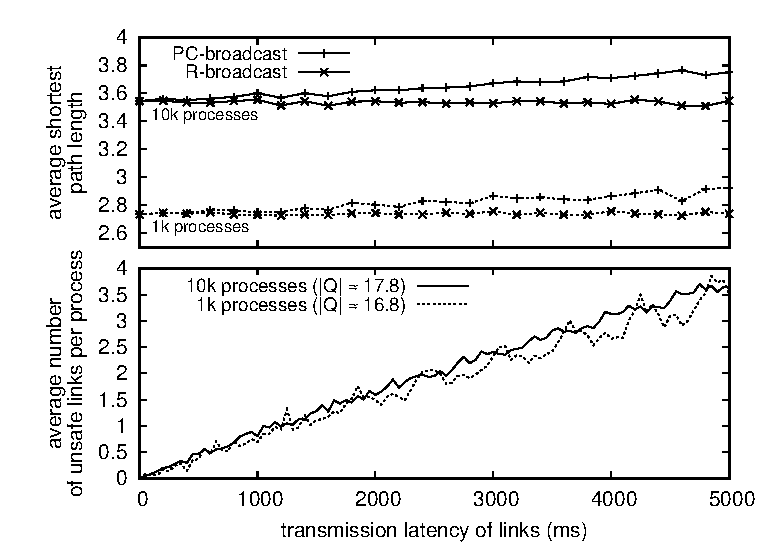
\includegraphics[width=0.7\textwidth]{img/delay.eps}
  \end{center}
  
  \vspace{-5pt}

  \small Messages arrive slightly later, for PC-broadcast temporarily forbids the use
  of new links. This is overlay-specific: removing an arc from a random-graph is
  not very impactful.

\end{frame}

\begin{frame}{Conclusion}
  
  PC-broadcast constitutes a simple and efficient implementation for causal broadcast
  in large and dynamic systems.

  Depending on the overlay network, the cost in terms of number of control
  messages and its negative impact on overlay's properties remains low.

  \vspace{2em}

  \begin{center}
  \begin{table}
    \begin{center}
      %\setlength{\tabcolsep}{3pt} % General space between cols (6pt standard)
\small
\begin{tabularx}{0.95\columnwidth}{@{}Xcccc@{}}
%  \toprule
  & \makecell{dynamic\\systems} & \makecell{message\\overhead} & \makecell{local space\\consumption} &  \makecell{delivery\\execution time} \\% \cmidrule{2-5}
  \hline\hline
%  objective & \cmark & $?<O(N)$ & $O(N)\leq \, ?$ & $? \leq O(W.N)$ \\ \hline\hline
  \textbf{our approach} & \textbf{\YES{\cmark}} & $\mathbf{O(1)}$ & $\mathbf{O(\NO{N})}$ & $\mathbf{O(1)}$ \\ 
%  \bottomrule
\end{tabularx}

%%% Local Variables:
%%% mode: latex
%%% TeX-master: "../paper"
%%% End:

    \end{center}
  \end{table}
  \end{center}


\end{frame}

\begin{frame}[standout]
  To be continued\ldots Removing the last monotonic upper bound on space complexity.  
  
  \vspace{2em}
  
  \small 
  \begin{table}
    \begin{tabularx}{0.312\columnwidth}{@{}c@{}}
      local space consumption \\
      \hline\hline
      $O(\NO{N}) \rightarrow O(?)$
    \end{tabularx}
  \end{table}
  
\end{frame}

\begin{frame}[standout]
  To be continued 2\ldots Retrieving partial order out of flattened orders.

  \vspace{2em}

  \begin{center}
    
\begin{tikzpicture}[scale=1]

%\normal

\newcommand\Y{-25pt};
\newcommand\X{25pt};
  
\draw[fill=black] (0, 0*\Y) node[left]{\footnotesize$a$} circle (1pt);
\draw[->](0*\X, 0*\Y) -- (0, 1*\Y);
\draw[fill=black] (0, 1*\Y) node[left]{\footnotesize$b$} circle (1pt);
\draw[->](0, 1*\Y) -- (0, 2*\Y);
\draw[fill=black] (0, 2*\Y) node[left]{\footnotesize$a'$} circle (1pt);

\draw[->] ( 1*\X, 1*\Y) -- ( 2*\X, 1*\Y);

\draw[fill=black] (3*\X, 0*\Y) node[left]{\footnotesize$a$} circle (1pt);
\draw[->](3*\X, 0*\Y) -- (3*\X, 1*\Y);
\draw[fill=black] (3*\X, 1*\Y) node[left]{\footnotesize$b$} circle (1pt);
\draw[->](3*\X, 0*\Y) -- (4*\X, 1*\Y);
\draw[fill=black] (4*\X, 1*\Y) node[right]{\footnotesize$a'$} circle (1pt);




\end{tikzpicture}
  \end{center}

\end{frame}


\begin{frame}[standout]
  
  \vspace{6em}

  Thanks!

  \vspace{5em}

  \small
  \faEnvelope ~ brice.nedelec@ls2n.fr

\end{frame}

\end{document}
